\chapter{Precision Systems}
	This chapter is focused on system-related aspects that are relevant to \de{precision systems}, in particular related to the abbe, sine and cosine errors, the kinematic design and the flexure hinges.
	
\section{Alignment: Abbe, sine and cosine errors}
	
	Alignment errors are arising every time we need to align a measurement system and the subject of study: we have to be aware of this kind of error in order to detect them and control/reduce them. In particular the \de{Abbe} error arise every time there's an offset between the object to be measured and the system that perform the measure.
	
	Doing a low-volume production (or with high added value products) it's possible to rely on a manual inspection held by highly trained technician in order to ensure a certain level of quality; considering instead a mass production a handmade check of each component it's not possible due to a fully automated manufacturing and assembly for which there is a little space for adjustment: repeatability and precision must be designed into the product in order to have a high quality.
	
	\paragraph{Abbe's error} Common alignment errors are related to the \textbf{Abbe's error} associated  to it's principle stating that \textit{"the measurement line shall be collinear with the line of motion"}.
	
	\begin{SCfigure}[1][bht]
		\centering
		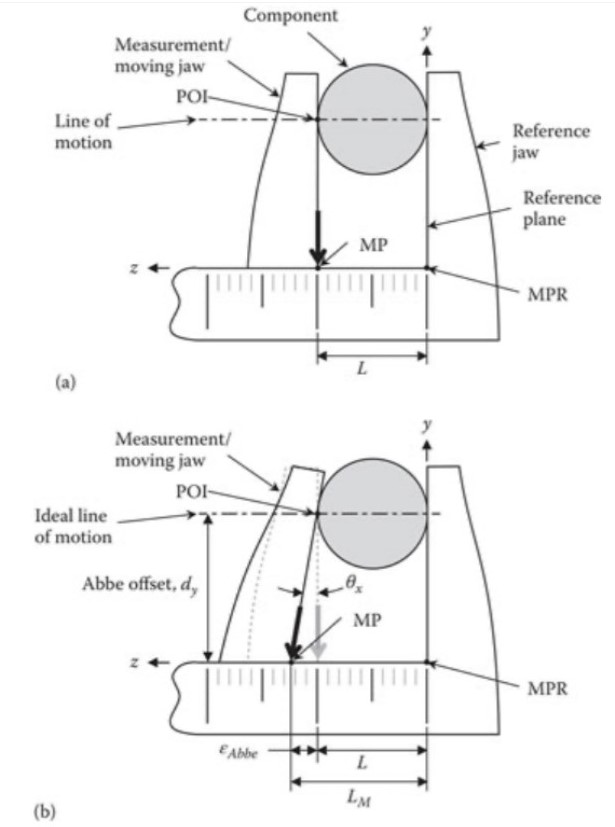
\includegraphics[width=6cm]{abbe-scheme}
		\caption{scheme used to understand the Abbe's error on a calliper. $(a)$ is a correct calliper while $(b)$ is affected by the error.} \label{fig:ps:abbescheme}
	\end{SCfigure}
	An example of this error can be seen in the calliper as in figure \ref{fig:ps:abbescheme}, where the goal is to measure the \textbf{Point of Interest} POI by reading the \textbf{Measurement Point} MP in respect to the Measurement Point \textbf{Reference} MPR. \\
	At a nominal level the two jaws of the calliper should be parallel, and so the point of interest is measured by only looking at the measurement point, but in reality misalignment are always present: this introduce an error $\abbe$ of the measurement point respect to the point of interest. Related to this error we can compute a linear relation but also an expression considering a second order term (that for low error alignment value $\theta_x$ can be neglected), obtaining
	\begin{equation}
		\abbe = d_y \tan\theta_x - \underbrace{L \left(\frac 1 {\cos\theta_x} - 1\right)}_\textrm{2nd ord. term}
	\end{equation}
	
	In reality things are even more complicated: Abbe's error are related to two angle in the 3D space, the so called \textbf{pith} and \textbf{yaw}
	\begin{equation}
	\begin{split}		
		\abbe & = d_y \tan\theta_x - L \left(\frac 1 {\cos\theta_x} - 1\right) + d_x \tan\theta_y - L \left(\frac 1 {\cos\theta_y} - 1\right) \\
		& = d_y \tan\theta_x + d_x\tan\theta_y - L\left( \frac 1 {\cos\theta_x} + \frac 1 {\cos\theta_y} - 2 \right)
	\end{split}
	\end{equation}
	
	\begin{SCfigure}[2][bht]
		\centering
		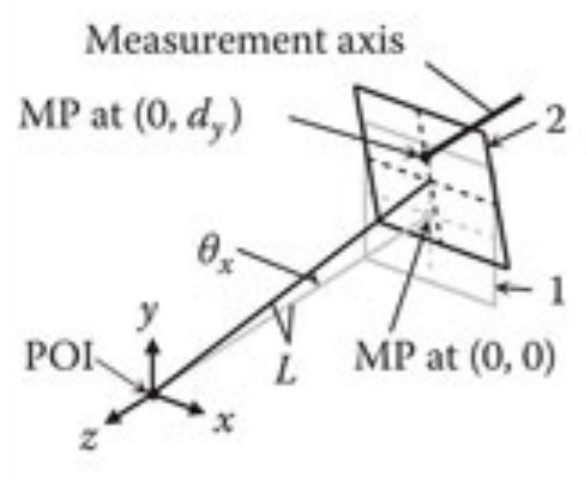
\includegraphics[width=3.5cm]{abbe-error}
		\caption{scheme used to understand the equation of the Abbe's error.} 
	\end{SCfigure}

	In order to eliminate the Abbe's error we can compensate by adding two more sensor (to determine $\theta_x,\theta_y$) that can determine the error $\abbe$. The same goal can be performed by analysing a sample problem: known it's value $L_m$, the computed measures is
	\[ L = L_m - d_y\tan\theta_x - d_x\tan\theta_y \]
	By evaluating this expression in two points (considering that an error, like $d_x\tan\theta_y$, can be consider negligible in respect to the other) by measuring an object more internal and external, we have a mathematical system that can be used in order to determine the unknown value $\theta_x$ and $L$. This method, in order to be successful, must consider that the angles $\theta_x$ and the length $L$ of the measure are invariant while changing the position of the sample.
	
	A smarter way to avoid the Abbe's error is just by doing a design choice minimizing the offset, so by making the line of motion collinear with the line of measurement.
	
	\paragraph{Cosine and sine error} The \de{cosine} error happens every time the measurement line is not parallel to the line of action. Considering the example of the measure of a length with a rule (as in figure \ref{fig:ps:cosineerror}) we can see that the measured length $L_m$ is different from the \textit{real} length $L$ of the object that we want to study, and in particular we can then evaluate the difference in order to define the cosine error $\varepsilon_{\cos}$:
	\begin{equation}
		L = L_m \cos\alpha \qquad \Rightarrow \quad \varepsilon_{\cos} = L_m - L = L_m \big(1-\cos\alpha\big)
	\end{equation}
	
	\begin{SCfigure}[1.3][bht]
		\centering
		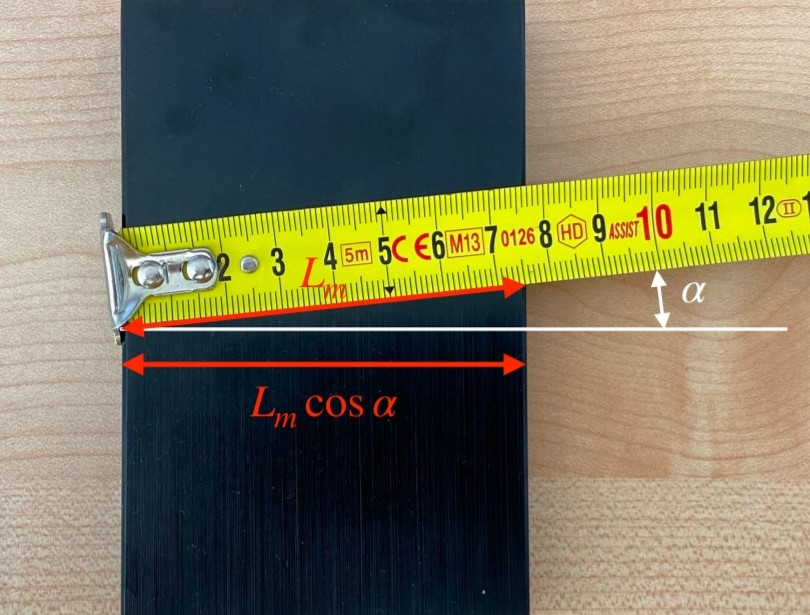
\includegraphics[width=5cm]{cosine-error}
		\caption{cosine error on a length measure.}  \label{fig:ps:cosineerror}
	\end{SCfigure}
	Extending the cosine error to a spatial environment we can compute  the error considering two angle $\alpha_x$ and $\alpha_y$ that can lead to an error:
	\begin{equation}
		\varepsilon_{\cos} = L_m\big(1-\cos\alpha_x\cos\alpha_y\big)
	\end{equation}
	\vspace{3mm}
	
	The \de{sine} error typically occurs when a physical contact is necessary for the measurement, like while dealing with the jaws of the calliper. By referring to figure \ref{fig:ps:sineerror} we can see that the error $\varepsilon_{\sin}$ is different in base of the geometry of the contact; considering as an example a flat-on-flat contact we can evaluate the error as
	\begin{equation}
		\varepsilon_{\sin} = \frac {w_z}2\sin\alpha_x + \frac{w_x}{2}\sin \alpha_z
	\end{equation}
	while considering instead a point contact the error reduces to the expression
	\begin{equation}
		\varepsilon_{\sin} = \frac {w_z}2\big(1-\cos\alpha_x\big) + \frac{w_x}{2}\big(1-\cos\alpha_z\big) = \frac{w_z}{2}\big(2-\cos\alpha_x-\cos\alpha_z\big)
	\end{equation}	
	
	
	\begin{SCfigure}[1.3][bht]
		\centering
		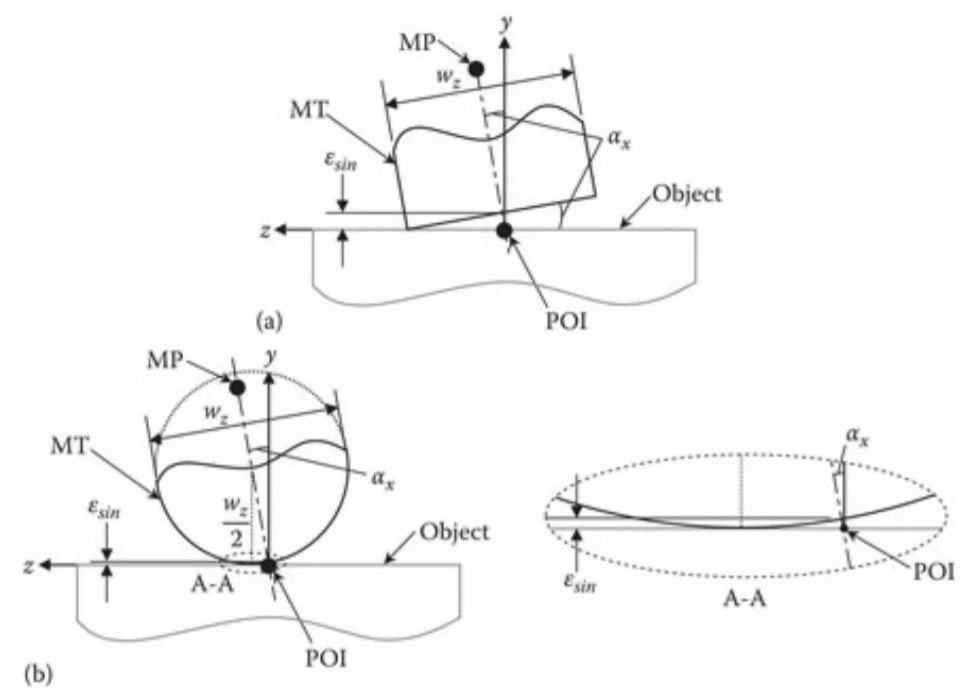
\includegraphics[width=5cm]{sine-error}
		\caption{sine error on a surface measure considering a flat-on-flat contact $(a)$ or a point contact $(b)$.}  \label{fig:ps:sineerror}
	\end{SCfigure}

	\paragraph{Alignment errors} In general Abbe's, cosine and sine errors are not mutually exclusive, so they can occur at the same time (Abbe's related to the offset, cosine due to a scale line not parallel to the  line of motion and the sine related to the angle between the moving jaw and the object).
	
	While designing measurement system it's important to determine all the specification that are useful to calculate the error factors that should be less then a decided value; this gives a suggestion on how to chose tolerances of the products.
	
	\begin{figure}[bht]
		\centering
		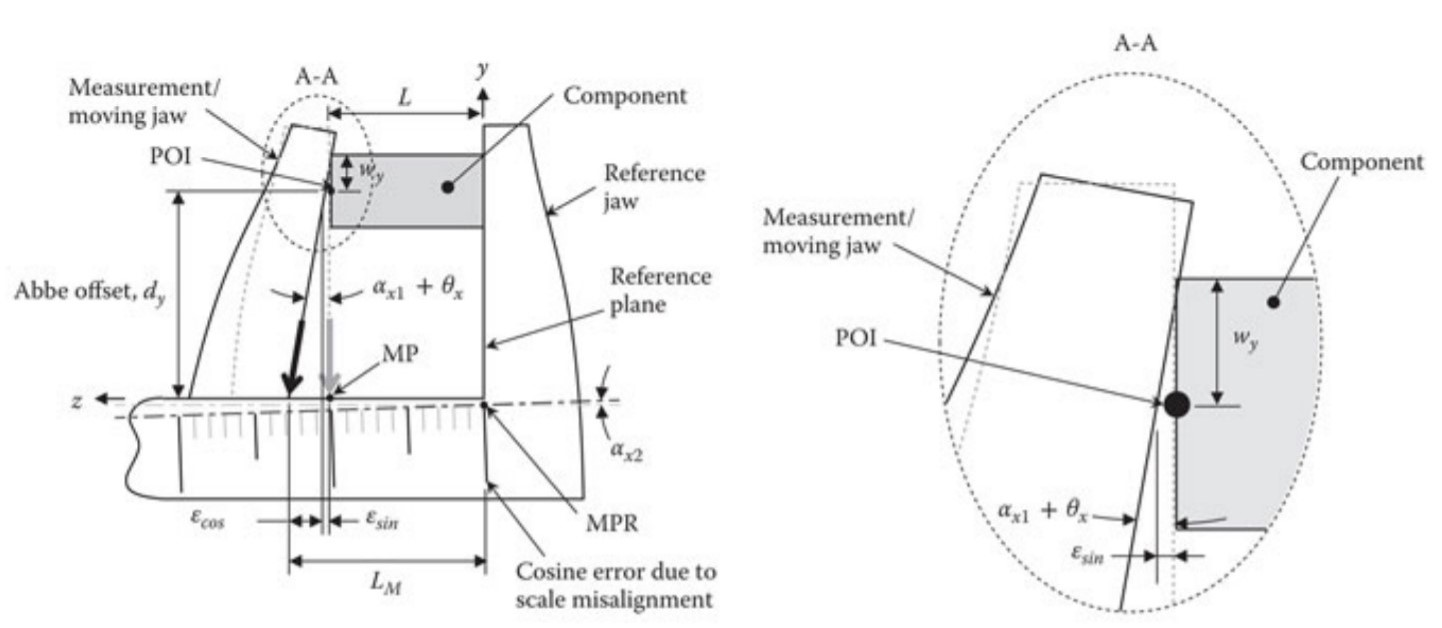
\includegraphics[width=10cm]{comb-errors}
		\caption{example of the combination of Abbe's, cosine and sine errors in a calliper.}
	\end{figure}
	
\section{Kinematics}
	
	In order to have a repeatable positioning it's important to minimize the internal stress by pursuing an isostatic design. When designing a system the kinematic analysis provides an understanding between the functional relationship between parts of mechanism, on how these parts are interconnected and how they move relative to each other.
	
	For example an unilateral constraint is represented by an inequality such $f(x,y,z) \geq 0$: in this step we usually consider bodies as \textbf{rigid}, so by considering part that are stiff enough in order to consider their deformation negligible in respect to the typical range of motion of the system. In precise machine it's important to consider all contact as rigid. \\
	In kinematic design we can assume that each	point of contact between two rigid bodies corresponds to a mutual constraint. In general if $f_j$ is the number of degrees of freedom of a joint $j$ having $n_{p_j}$ lowest number of contact point, than it's true that
	\begin{equation}
	\begin{split}
		\textrm{planar kinematics:}& \qquad f_j = 3 - n_{p_j} \\
		\textrm{spatial kinematics:}& \qquad f_j = 6 - n_{p_j} \\
	\end{split}
	\end{equation}
	
	Considering the more complex scenario of two line (straight or arcuate) contact, this is kinematically equivalent to two point constraints applied to any two different points along the contact line. 
	
	\begin{SCfigure}[2][bht]
		\centering
		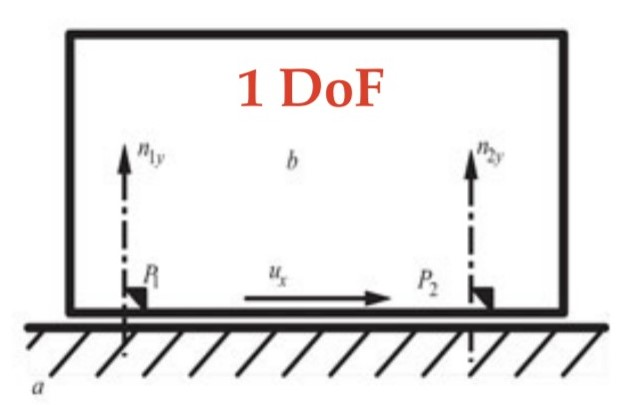
\includegraphics[width=3.5cm]{planar-contact}
		\caption{the contact of a body with straight line on a straight surface leads to two point constrains in order to have 1 degrees of freedom.}
	\end{SCfigure}
	
	\paragraph{Mobility of mechanisms} Considering now  a combination of $n$ rigid bodies constrained by $j$ joints can lead to a movable or immovable system. The net mobility of the mechanism is its number of degrees of freedom and can be calculated according to Tchebytchev as
	\begin{equation}
		M = D\big(n-1-j\big) +\sum_i f_i = D\big(n-1\big) -\sum_j n_{p_j}
	\end{equation}
	where $D= 6$ for spatial mechanisms while $D= 3$ for planar kinematics. If $M>0$ then the mechanism is movable, for $M = 0$ the system is immovable while $M < 0$ it's over-constrained and so, in a real application, the structure will be subjected to unknown internal stresses that cannot be quantified (and so leading to imprecision).
	
	The Tchebytchev should be used with caution when dealing with bodies that present singularities	
	
	
	
	
	
	
	
	
	
	
	
	
	
	
	
	
	
	
	
	
	
	
	
	
	
	
	
	
	
	

\section{Flexure hinges}
	
	
	
	
	
	
	
	
	
	
	
	
	
	
	
	
	
	
	
	
	
	
	
	
	
	
	
	
	
	
	
	
	
	
	
	
	
	
	
	
	
	
	
	